\documentclass[12pt]{article}
\usepackage[utf8]{inputenc}
\usepackage{graphicx}
\usepackage{amsmath}
\usepackage{xcolor}
\usepackage{listings}
\usepackage[margin=1in]{geometry}
\usepackage{hyperref}
\usepackage{caption}
\usepackage{subcaption}
\usepackage{titlesec}
\usepackage{booktabs}
\usepackage{float} % Added for better figure positioning

\definecolor{codebg}{rgb}{0.95,0.95,0.95}
\definecolor{myblue}{rgb}{0,0.3,0.6}

\lstset{
    backgroundcolor=\color{codebg},
    basicstyle=\ttfamily\small,
    breaklines=true,
    frame=single,
    numbers=left,
    numberstyle=\tiny\color{gray},
    keywordstyle=\color{myblue},
    commentstyle=\color{green!50!black},
    stringstyle=\color{red},
    showstringspaces=false,
    tabsize=4
}

\title{Morphology Operators Implementation}
\date{\today}

\begin{document}

\maketitle

\begin{abstract}
This document demonstrates the implementation of basic morphology operations (erosion and dilation) using NumPy, including image padding and kernel processing. The code shows each step of the morphological operations with clear outputs.
\end{abstract}

\section{Libraries Used}
\begin{itemize}
    \item \texttt{numpy}: For numerical operations and array manipulation (core library for image processing)
\end{itemize}

\section{Step-by-Step Process}

\subsection{Step 1: Import Libraries}
\begin{lstlisting}[language=Python]
import numpy as np
\end{lstlisting}

\subsection{Step 2: Define Image with numpy}
Create a sample 8x8 grayscale image as a NumPy array for processing.

\begin{lstlisting}[language=Python]
image = np.array([[10, 10, 10, 20, 10, 10, 20, 10],
                  [10, 20, 20, 20, 20, 20, 20, 10],
                  [10, 10, 10, 20, 10, 20, 20, 10],
                  [10, 10, 20, 30, 10, 20, 30, 10],
                  [10, 10, 30, 10, 10, 30, 10, 20],
                  [20, 10, 30, 10, 30, 20, 20, 10],
                  [20, 20, 20, 20, 10, 10, 20, 10],
                  [20, 20, 30, 20, 20, 30, 10, 30]], dtype=np.uint8)
\end{lstlisting}

\subsection{Step 3: Reflect Padding}
Add border padding to handle edge pixels during morphological operations.

\begin{lstlisting}[language=Python]
def reflect_padding(image, padding_size):
    height, width = image.shape
    padded_image = np.zeros((height + padding_size*2, width + padding_size*2), dtype=image.dtype)
    
    # Center
    padded_image[padding_size:height+padding_size, padding_size:width+padding_size] = image
    
    # Borders
    for i in range(padding_size):
        padded_image[i, padding_size:width+padding_size] = image[0, :]
    
    for i in range(height+padding_size, height+padding_size*2):
        padded_image[i, padding_size:width+padding_size] = image[-1, :]
    
    for j in range(padding_size):
        padded_image[padding_size:height+padding_size, j] = image[:, 0]
    
    for j in range(width+padding_size, width+padding_size*2):
        padded_image[padding_size:height+padding_size, j] = image[:, -1]
    
    # Corners
    padded_image[:padding_size, :padding_size] = image[0, 0]
    padded_image[:padding_size, width+padding_size:] = image[0, -1]
    padded_image[height+padding_size:, :padding_size] = image[-1, 0]
    padded_image[height+padding_size:, width+padding_size:] = image[-1, -1]
    
    return padded_image

padded_image = reflect_padding(image, 1)
\end{lstlisting}

% Print Output immediately after the code it belongs to
\begin{figure}[H]
    \centering
    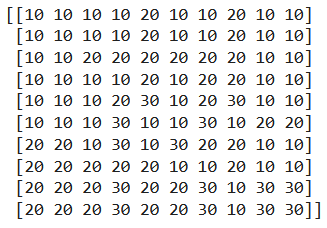
\includegraphics[width=0.4\textwidth]{padded_output.png}
    \caption{Padded image output (10x10 array)}
    \label{fig:padded}
\end{figure}

\subsection{Step 4: Define Kernel}
Create a 3x3 kernel for morphological operations.

\begin{lstlisting}[language=Python]
kernel = np.array([[1, 1, 1],
                   [1, 0, 0],
                   [1, 0, 0]], dtype=np.uint8)
\end{lstlisting}

\subsection{Step 5: Calculate Erosion}
Implement erosion operation which shrinks bright regions in the image.

\begin{lstlisting}[language=Python]
def calculate_erosion(image, kernel):
    height, width = image.shape
    kernel_height, kernel_width = kernel.shape
    kernel_height //= 2
    kernel_width //= 2

    result_image = np.zeros((height - 2*kernel_height, width - 2*kernel_width), dtype=image.dtype)
    for i in range(kernel_height, height - kernel_height):
        for j in range(kernel_width, width - kernel_width):
            matrix = image[i-kernel_height:i+kernel_height+1, j-kernel_width:j+kernel_width+1]
            multiplied = matrix * kernel
            multiplied = multiplied.flatten().tolist()
            while 0 in multiplied:
                multiplied.remove(0)
            result_image[i - kernel_height, j - kernel_width] = min(multiplied)
    return result_image

erosion = calculate_erosion(padded_image, kernel)
\end{lstlisting}

% Print Output immediately after erosion code
\begin{figure}[H]
    \centering
    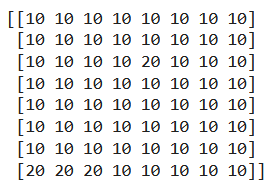
\includegraphics[width=0.4\textwidth]{erosion_output.png}
    \caption{Erosion result (8x8 array)}
    \label{fig:erosion}
\end{figure}

\subsection{Step 6: Calculate Dilation}
Implement dilation operation which expands bright regions in the image.

\begin{lstlisting}[language=Python]
def calculate_dilation(image, kernel):
    height, width = image.shape
    kernel_height, kernel_width = kernel.shape
    kernel_height //= 2
    kernel_width //= 2

    result_image = np.zeros((height - 2*kernel_height, width - 2*kernel_width), dtype=image.dtype)
    for i in range(kernel_height, height - kernel_height):
        for j in range(kernel_width, width - kernel_width):
            matrix = image[i-kernel_height:i+kernel_height+1, j-kernel_width:j+kernel_width+1]
            multiplied = matrix * kernel
            multiplied = multiplied.flatten().tolist()
            while 0 in multiplied:
                multiplied.remove(0)
            result_image[i - kernel_height, j - kernel_width] = max(multiplied)
    return result_image

dilation = calculate_dilation(padded_image, kernel)
\end{lstlisting}

% Print Output immediately after dilation code
\begin{figure}[H]
    \centering
    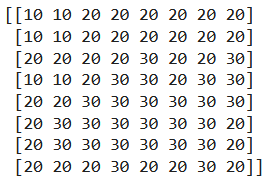
\includegraphics[width=0.4\textwidth]{dilation_output.png}
    \caption{Dilation result (8x8 array)}
    \label{fig:dilation}
\end{figure}

\section{Technical Explanations}

\subsection{Morphological Operations}
\begin{itemize}
    \item \textbf{Erosion}: Reduces bright regions by taking the minimum value under the kernel
    \item \textbf{Dilation}: Expands bright regions by taking the maximum value under the kernel
    \item \textbf{Kernel}: A small matrix used to probe the image (structuring element)
    \item \textbf{Padding}: Necessary to handle border pixels during convolution
\end{itemize}

\subsection{Implementation Notes}
\begin{itemize}
    \item The kernel is asymmetric (non-uniform weights)
    \item Zero values in kernel are ignored in min/max calculations
    \item Reflect padding helps reduce border artifacts
    \item Operations are implemented manually for educational purposes
\end{itemize}

\begin{center}
    \href{https://github.com/AsadiAhmad/Morphology-Operators}{
        \includegraphics[width=0.2\textwidth]{github_logo.png} \\
        \texttt{https://github.com/AsadiAhmad/Morphology-Operators}
    }
\end{center}

\end{document}